\documentclass[11pt]{article}

\usepackage[lined,boxed,linesnumbered]{algorithm2e}
\usepackage{amsmath}
\usepackage{graphicx}

\begin{document}
\author{Mohit Sharma}
\title{Latex Documentation}
\maketitle

\section{Multiplication of two long numbers}

\subsection{Problem:}
 Multiplying two numbers given as array of digits forming them. Maximum number of digits 
 in each number is n. \\

\subsection{ Solution: }
We solve the multiplication problem through the approach adopted in school. We save the first number as a string in array $A$, second number as string in array $B$.We store result of multiplication in an array $C$. We start from last element (before '/0') of array $B$. Keep multiplying it with digits of number $A$ starting again from the last element and going till the first digit of $A$. At each step we store the result of multiplication $(mod 10)$ in same cell and carry  (result/10) to next step.\\
{Note:} The result C is in reverse order.\\
Then we do the same with the second-last element of B and this time, we start adding result from secondlast element of C. and at each step we start from one element ahead than previous time.
In the end, we will be left with answer to multiplication in reverse order.\\\\

\begin{algorithm}[!h]
\KwData{Input will be two arrays $ A[0..n-1]$ and $ B[0..n-1]$. We will use an extra array $C[0..(2n-1)] $ to store the result at each step and hence the result of multiplication after final step.}
\KwResult{The result will be multiplication of two given number in digit form in array $C$}
Set all elements of $C$ to be zero.\\
Get number of digits of $A$ and $B$, say it equals $a$ and $b$ respectively.\\
\For{$ i\leftarrow (b-1) $ \KwTo $ 0 $}{
	k=$(b-1)$ - $i$;\\
	\For{$j\leftarrow (a-1)$ \KwTo $ 0 $}{
	$result$= $B[i]*A[j]$;\\
	$C[k]$= ($C[k]$+$carry+result$) \% 10;\\
	$carry$= ($C[k]$+$carry+result$)/10;\\
	$k$++;\\
	}
	C[k]=C[k] + carry;
	}
Reverse array $C$;\\
return array$C$\\
\caption{Algorithm for multiplying two long numbers}
\end{algorithm}
\begin{figure}[!h]
\centerline{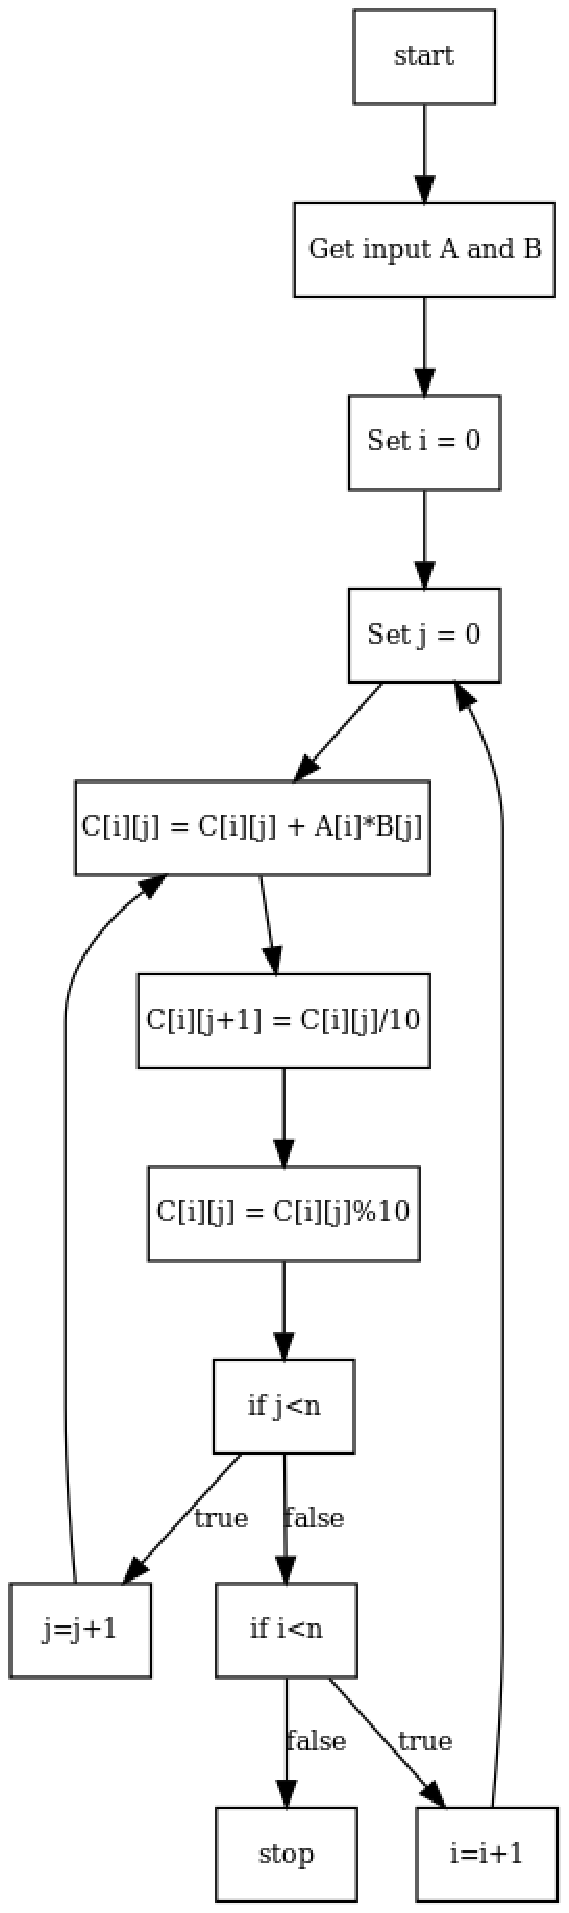
\includegraphics[scale=0.6]{flowc}}
\caption{Algorithm explained through flowchart}
\end{figure}


\subsection{Analysis of Time Complexity of the Algorithm}
Algorithm 1 executes ``for'' loop on $i$, $b-1$ times, and in each iteration it runs another for loop on $j$, $a-1$ times doing some constant number of operations. \\
Hence the total number of operations executed are $k*a*b$ where $k$ is a constant.Maximum value of a and b can be $n$ and hence worst case time complexity is $k*(n^2)$ or O$(n^2)$.

\end{document}
